\documentclass{beamer}
%\usepackage[latin1]{inputenc}
\usepackage{amsmath}
\usepackage{amssymb}
\usepackage{verbatim}
%\usepackage{cite}
\usepackage{booktabs}
\usepackage{multirow}
\usepackage{fancyvrb}
\usepackage{color}
\usepackage[vlined,ruled,commentsnumbered]{algorithm2e}
\usepackage{tikz}

\DeclareMathOperator{\probability}{Pr}
\DeclareMathOperator*{\argmax}{arg\,max}
\DeclareMathOperator*{\argmin}{arg\,min}


\usetheme{Warsaw}
%\usetheme{Copenhagen}

\title{Continuous-time systems 1}
%\subtitle{A Library for Ensemble Learning Using Support Vector Machines}
%\author{Marc~Claesen}
%\institute{ESAT-STADIUS, KU~Leuven \\ iMinds Medical IT Department}

\definecolor{blueish}{rgb}{0.3,0.3,0.7}

\AtBeginSection[]
{
\begin{frame}<beamer>
\frametitle{Outline}
\tableofcontents[currentsection]
\end{frame}
}

%\AtBeginSubsection[]
%{
%\begin{frame}<beamer>
%\frametitle{Outline}
%\tableofcontents[currentsubsection]
%\end{frame}
%}

%\AtBeginSubsubsection[]
%{
%\begin{frame}<beamer>
%\frametitle{Outline}
%\tableofcontents[currentsubsection]
%\end{frame}
%}

%% let pdflatex show eps figs
\newif\ifpdf
\ifx\pdfoutput\undefined
\pdffalse
\else
\pdfoutput=1
\pdftrue
\fi
\ifpdf
\usepackage{graphicx}
\usepackage{epstopdf}
%nessim
\epstopdfsetup{suffix=}
\DeclareGraphicsRule{.eps}{pdf}{.pdf}{`epstopdf #1}
\pdfcompresslevel=9
\else
\usepackage{graphicx}
\fi

\begin{document}
%\nocite{*}

\begin{frame}
\titlepage
\end{frame}

\begin{frame}
\tableofcontents
\end{frame}

\section{Linear differential equations}

\begin{frame}
\frametitle{Linear differential equations: definitions 1/2}
Linear differential equations (LDE) are of the following form:
\begin{equation*}
L[y(t)] = f(t),
\end{equation*}
where $L$ is some linear operator. \\ \pause
\ \newline
The linear operator $L$ is of the following form:
\begin{equation*}
L_n(y) = \sum_{i=0}^{n} A_i(t) \frac{d^{n-i}y}{dt^{n-i}},
\end{equation*}
with given functions $A_{1:n}$.\\ \pause
\ \newline
The \textbf{order of a LDE} is the index of the highest derivative of $y$.
\end{frame}

\begin{frame}
\frametitle{Linear differential equations: definitions 2/2}
\begin{equation*}
L_n(y) = \sum_{i=0}^{n} A_i(t) \frac{d^{n-i}y}{dt^{n-i}} = f(t).
\end{equation*}
\begin{itemize}
\item $y$ is a scalar function $\rightarrow$ \textbf{ordinary differential equation} (ODE) \pause
\item $y$ is a vector function $\rightarrow$ \textbf{partial differential equation} (PDE) \\
\ \pause
\item $f = 0$ $\rightarrow$ \textbf{homogeneous equation} \\
$\rightarrow$ solutions are called \textbf{complementary functions} \\
\ \pause
\item if $A_{0:n}(t)$ are constants (ie. not functions of time), the LDE is said to have \textbf{constant coefficients}
\end{itemize}
\end{frame}

\begin{frame}
\frametitle{Example: radioactive decay 1/2}
Let $N(t)$ be the number of radioactive atoms at time $t$, then:
\begin{equation*}
\frac{dN(t)}{dt} = - k N(t),
\end{equation*}
for some constant $k>0$. \\ \pause
\ \newline
This is a first order homogeneous LDE with constant coefficients.
\end{frame}

\begin{frame}
\frametitle{Example: radioactive decay 2/2}
\begin{figure}
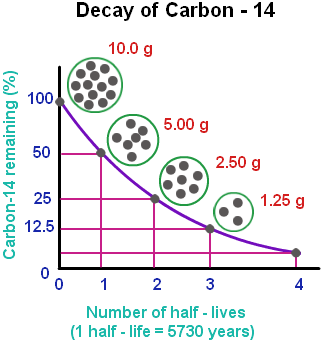
\includegraphics[width=0.5\textwidth]{decay-of-carbon-14.png}
\end{figure}
\end{frame}

\begin{frame}
\frametitle{Solving homogeneous LDEs with constant coefficients 1/3}
Solutions of LDEs must be of the form $e^{zt}$ with $z \in \mathbb{C}$. \\
\pause
\ \newline
We assume an LDE with constant coefficients:
\begin{equation*}
\sum_{i=0}^n A_i y^{(n-i)} = 0.
\end{equation*}
\ \pause
Replacing $y = e^{zt}$ leads to:
\begin{equation*}
\sum_{i=0}^n A_i z^{n-i} e^{zt} = 0
\end{equation*}
\ \pause
Dividing by $e^{zt}$ yields the $n$th order \textbf{characteristic polynomial}:
\begin{equation*}
F(z) = \sum_{i=0}^n A_i z^{n-i} = 0.
\end{equation*}
\end{frame}

\begin{frame}
\frametitle{Solving homogeneous LDEs with constant coefficients 2/3}
Characteristic equation:
\begin{equation*}
F(z) = \sum_{i=0}^n A_i z^{n-i} = 0.
\end{equation*}
\pause
\begin{enumerate}
\item Solving the polynomial $F(z)$ yields $n$ zeros $z_1$ to $z_n$.
\item Substituting a given zero $z_i$ into $e^{zt}$ gives a solution $e^{z_it}$.
\end{enumerate}
\ \newline
\pause
Homogeneous LDEs obey the superposition position: \\
$\rightarrow$ any linear combination of solutions $e^{z_1t}$,\ldots,$e^{z_nt}$ is a solution \pause \\
$\rightarrow$ $e^{z_1t}$,\ldots,$e^{z_nt}$ form a basis of the solution space of the LDE \\
\pause 
\ \newline
The specific linear combination depends on initial conditions.
\end{frame}


\begin{frame}
\frametitle{Solving homogeneous LDEs with constant coefficients 3/3}
Example:
\begin{equation*}
y^{(4)}(t) - 2 y^{(3)}(t) + 2 y^{(2)}(t) - 2 y^{(1)}(t) + y(t) = 0.
\end{equation*}
\pause
This is a 4th order homogeneous LDE with constant coefficients.\\
\ \newline
\pause
The corresponding characteristic equation:
\begin{equation*}
F(z) = z^4 - 2z^3 + 2z^2 - 2 z + 1 = 0.
\end{equation*}
\pause
The zeros of $F(z)$ are ($j=\sqrt{-1}$):
\begin{equation*}
z_1 = j, \quad z_2 = -j, \quad z_{3, 4} = 1.
\end{equation*}
\pause
These zeros correspond to the following basis functions $t$:
\begin{equation*}
 e^{jt}, \quad e^{-jt}, \quad e^t, \quad te^t.
\end{equation*}
\end{frame}

\section{Laplace transform}

\begin{frame}
\frametitle{The Laplace transform}
The Laplace transform of $f(t)$, for all real numbers $t\geq 0$:
\begin{equation*}
F(s) = \mathcal{L}\big\{f(t)\big\} = \int_0^\infty e^{-st} f(t) dt.
\end{equation*}
\pause
The parameter $s = \sigma + j\omega$ is the complex number frequency.\\ \pause
\ \newline
The initial value theorem states $f(0^+) = \lim_{s\rightarrow\infty} sF(s)$. \\
\pause
\ \newline
The final value theorem states $f(\infty) = \lim_{s\rightarrow0} sF(s)$, \\
if all poles of $sF(s)$ are in the left half plane (ie. real part $<0$).
\end{frame}

\begin{frame}
\frametitle{Important properties of the Laplace transform}
\centering
\begin{tabular}{lcc}
\textbf{property}	& \textbf{time domain}	& \textbf{$s$-domain} \\
\midrule
linearity	& $af(t)+bg(t)$ & $aF(s) + bG(s)$ \\ \pause
\ \\
differentiation	& $f^{(1)}(t)$	& $s F(s) - f(0)$ \\ \pause
\ \\
integration	& $\int_0^t f(\tau)d\tau = (u*f)(t)$	&	$\frac{1}{s}F(s)$ \\ \pause
\ \\
convolution	& $(f * g)(t)=\int_0^t f(\tau)g(t-\tau)d\tau$	& $F(s)\cdot G(s)$ \\ \pause
\ \\
time scaling	& $f(at)$	& $\frac{1}{a}F(\frac{s}{a})$ \\ \pause
\\
time shifting	& $f(t-a)u(t-a)$	& $e^{-as} F(s)$ \\ \pause
\end{tabular} \\
with $u(t)=\int_\infty^t \delta(t)dt$ (Heaviside) and $\delta(t)$ the Dirac delta.
\end{frame}


\begin{frame}
\frametitle{Inverse Laplace transform}
The inverse Laplace transform converts $s$-domain to time domain:
\begin{equation*}
f(t) = \mathcal{L}^{-1}\{F(s)\} = \frac{1}{j2\pi}\int_{\gamma-jT}^{\gamma+jT} e^{st} F(s) ds.
\end{equation*}
\pause
\ \newline
Practically, the inverse Laplace transform takes two steps:
\begin{enumerate}
\item write $F(s)$ in terms of partial fractions
\item transform each term in the partial fraction \\ based on tables of $s$/$t$-domain pairs \\ (course notes p 4.32-4.33)
\end{enumerate}
\end{frame}

\section{Solving LDEs with the Laplace transform}

\begin{frame}
\frametitle{Solving LDEs with the Laplace transform 1/3}
The Laplace transform can be used to solve LDEs with given initial conditions 
(the previous approach gave us the basis functions). \\
\pause
\ \newline
This is done by using the following property (differentiation):
\begin{align*}
\mathcal{L}\{f^{(1)}\} &= s F(s) - f(0), \\
\mathcal{L}\{f^{(2)}\} &= s^2 F(s) -s f(0) - f^{(1)}(0).
\end{align*}
\pause
Via induction, the Laplace transform of the $n$th order derivative:
\begin{equation*}
\mathcal{L}\{f^{(n)}\} = s^n F(s) - \sum_{i=1}^n s^{n-i}f^{(n-i)}(0)
\end{equation*}
\end{frame}

\begin{frame}
\frametitle{Solving LDEs with the Laplace transform 2/3}
\begin{equation*}
\mathcal{L}\{f^{(n)}\} = s^n F(s) - \sum_{i=1}^n s^{n-i}f^{(n-i)}(0)
\end{equation*}
\pause
We want to solve the following LDE:
\begin{align*}
\sum_{i=0}^{n} A_i y^{(n-i)}(t) &= f(t), \\
y^{(i)}(0) &= c_i \quad \forall i=0\ldots n.
\end{align*}
\pause
Via the linearity of the Laplace transform:
\begin{equation*}
\sum_{i=0}^{n} A_i \mathcal{L}\{y^{(n-i)}(t)\} = \mathcal{L}\{f(t)\} 
\end{equation*}
\end{frame}

\begin{frame}
\frametitle{Solving LDEs with the Laplace transform 3/3}
\begin{align}
\sum_{i=0}^{n} A_i \mathcal{L}\{y^{(n-i)}(t)\} &= \mathcal{L}\{f(t)\}  \label{firsteq} \\
\mathcal{L}\{f^{(n)}\} &= s^n F(s) - \sum_{i=1}^n s^{n-i}f^{(n-i)}(0) \label{secondeq}
\end{align}
\pause
Expanding Eq.~\eqref{secondeq} into \eqref{firsteq} yields:
\begin{equation*}
Y(s)\sum_{i=0}^n A_i s^i - \sum_{i=1}^n \sum_{j=1}^i A_i s^{i-j}y^{j-1}(0) = F(s)
\end{equation*}
\pause
The solution in the time domain is obtained via the inverse Laplace transform: $y(t) = \mathcal{L}^{-1}\{Y(s)\}$.
\end{frame}


\end{document}
